\documentclass[lnbip]{svmultln}

\usepackage{makeidx}
\usepackage{graphicx}
\usepackage{url}

\newcommand{\footnoteremember}[2]{
  \footnote{#2}
  \newcounter{#1}
  \setcounter{#1}{\value{footnote}}
}
\newcommand{\footnoterecall}[1]{
  \footnotemark[\value{#1}]
} 

\begin{document}

\mainmatter

\title{Open Source and Agile Methods:\\Two worlds closer than it
  seems}

\titlerunning{Open Source and Agile Methods}

\author{}
%\author{Hugo Corbucci\inst{1} and Alfredo Goldman\inst{1}}

%\authorrunning{Hugo Corbucci et al.}

%\tocauthor{Hugo Corbucci, Alfredo Goldman}

\institute{}
%\institute{Instituto de Matem\'{a}tica e Estat\'{i}stica (IME)\\
%  Universidade de S\~{a}o Paulo (USP) - Brazil\\
%  \email{corbucci@ime.usp.br} and \email{gold@ime.usp.br} }
 
\maketitle

\begin{abstract}
  Agile methods and open source software communities have different
  approaches to produce high quality and successful software. However
  agile methodologies are not very diffused in open source communities
  nor the members of those communities follow many agile
  practices.

% TODO Mais abstract

  \keywords{agile software development, open source software,
    distributed agile, free software, software libre }
\end{abstract}

\section{Introduction}

Typical Open Source (OS) projects (the scope of OS project will be
narrowed according to Section \ref{sec:scope}) usually receive the
collaboration of many geographically distant
people~\cite{report:dempsey1999}. At first glance, this argument could
indicate that such projects are not candidates for the use of agile
methods since some basic values seem to be missing. In this case, the
distance and diversity separating developers deteriorates
communication, a very important value within agile methods. However,
it is common to identify some principles presented by the agile
manifesto \cite{url:agilemanifesto} on many OS software
projects. Parts of the manifest such as being ready for changes,
working with continuous feedback, respecting collaborators and users,
delivering working features and facing challenges can be naturally
found in the Free, Libre, Open Source Software (FLOSS)
communities~\cite{gabriel2005}.

During a workshop \cite{conference:oopsla2007} held at OOPSLA 2007
celebrating 20 years from the publication of ``No Silver
Bullets''\cite{brooks1987}, agile methods and OS software development
were mentioned as two failed silver bullets having both brought great
benefits to the software community. During that workshop, someone
asked if the use of several failed silver bullets simultaneously could
not raise production levels by an order of magnitude. This work
analyses parts of those environments to observe if a merging between
agile methods and OS development could have benefical effects to
software development.

This work is structured as follows. Section \ref{sec:scope} defines
what is meant by FLOSS and agile methods in this paper. Section
\ref{sec:relation} shows where agile methods and FLOSS development are
close to each other and where they diverge. Section \ref{sec:surveys}
presents two surveys elaborated to try to identify communication
issues and possible tools to minimize the problems of each
community. Section \ref{sec:results} presents the results of the
survey while Section \ref{sec:conclusion} concludes and provides
suggestions for future works.

\section{Scope}
\label{sec:scope}

The FLOSS environment as well as the agile methodologies both
comprehend such a wide variety of projects, people and contexts that
it is very hard to cover all of them. Therefore it is necessary to
first define which part of each community will be analysed in this
work.
\\

In this work, we will thread any software engineering method that
follows the principles of the agile manifesto
\cite{url:agilemanifesto} as an agile method. However the text will be
guided by the most known methods such as eXtreme Programming
\cite{XP2002}, Scrum \cite{schwaber2004} and the Crystal family
\cite{cockburn2002}. Closely related ideas will also be mentioned from
the wider Lean philosophy \cite{ohno1998} and its application to
software development \cite{poppendieck2005}.
\\

The terms ``open source software'' and ``free software'' will be
considered the same in this work although they have some differences
in their specific contexts \cite{fogel2005}. Projects will be said to
be open source (or free) if their source code is available and
modifiable by anyone with the required technical knowledge, without
prior consent from the original author and without any charge.

OS projects essentially controlled by a single company fall out of the
scope of this work. The reason for such reduction of scope is that
projects controlled by companies, whether they have a public source
code and accept external collaboration or not, can be run with any
software engineering method established in the company since it can be
enforced to the employees of this company.

Considering this scope, it is important to characterize the people
involved in such kind of projects. In 2002, the FLOSS Project
\cite{url:flossproject} published a report about a survey they
conducted regarding FLOSS contributors. Their collected data
\cite{url:flossdata} shows that 78.77\% of the contributors are
employed or self-employed (question 42) and that only 50.82\% of the
OS community are software developers while 24.76\% do not earn their
main income with software development (question 10).  In addition to
those results, the survey presents the fact that 78.78\% of the
collaborators consider their OS tasks more joyful (question 22.2) than
their regular activities and 42.3\% also consider them better
organized (question 22.4). As an outcome of those results, we could
say that OS contributors perceive their activities both pleasurable
and effective.

% TODO Rever essas porcentagem para trocar por algo mais interessante

Another survey \cite{reis2003} points out that 74\% of open source
projects have teams with up to 5 people and 62\% of the contributors
work with each other over the Internet and have never met physically.

Considering such characterization of the FLOSS community, the next
section presents what is the relation between such development
environment with the ideas and guidelines of agile methodologies.

\section{How closely related are Open source and Agile?}
\label{sec:relation}

In Martin Fowler's first version of ``The New Methodology''
\cite{url:fowler2000orig}, he included OSS development as part of the
new methodology of software development along with now well known
agile methods. He decided to remove it from the final article because
the FLOSS environment is so big and spread that any attempt to
characterize the development process would undoubtedly fail on a given
environment.

Afterwards, in 2002, Warsta \cite{warsta2002} published a review about
agile software development methods including and discussing FLOSS as
an agile method.  However, he stresses that FLOSS development is not a
precise method and evolves differently for each project. Indeed, Eric
Raymond's description of the development process from ``The Cathedral
and the Bazaar'' \cite{raymond1999} is closer to an experience report
than to the description of a process with guidelines and
practices. Nevertheless, Raymond's text presents several actions that
could be related to the agile manifesto \cite{url:agilemanifesto} and
are common in other FLOSS projects.

FLOSS communities are, by definition, a group of people gathered
around a FLOSS project. A working and useful software project attracts
individuals to collaborate and evolve the
software~\cite{crowston2002}. It is the people's interactions that
will define the development process, tools and even the goals of the
software. FLOSS projects that do not evolve to fit the needs of its
community are abandoned in a highly competitive environment where the
best (in certain criteria) gains adopters in a thin line between
success and oblivion.

From such aspects, FLOSS projects share a lot with the values
presented by agile methods. The practices are also quite similar. Eric
Raymond quotes Linus Torvalds about two specific development policy
for the Linux Kernel~\cite{raymond1999}.
\begin{quote}
  \begin{enumerate}
  \item[7.] Release early. Release often. And listen to your
    customers.
  \item[8.] Given a large enough beta-tester and co-developer base,
    almost every problem will be characterized quickly and the fix
    will be obvious to someone.
  \end{enumerate}
\end{quote}

The first policy hints for an iterative and short development process
with frequent feedback input. The second one points to a large amount
of test done frequently. Those ideas are core principles for agile
methods and largely applied to several successful FLOSS projects.
% TODO Referencias

We can, therefore, state that the FLOSS community have a culture that
is similar to the one of the agile community. Given that there is such
proximity between agile methods and FLOSS development, it must not be
forgotten that the environments in which each solution out stands are
quite different.

Open source software is stronger when it comes to products that
``scratch a developer's itch'' \cite{fitzgerald2000}, i.e. a product
in which the developer can be the user. Such product evolves across
the Internet gathering volunteers interested in such development by
releasing versions of the software frequently.

Agile methods come from industry consultants with focus on business
problems and customer satisfaction through frequent high quality
releases. To achieve such goal, an ideal agile team needs motivated
competent people closely gathered with freedom to improve their
environment and process to enable what Cockburn calls osmotic
communication \cite{cockburn2004}.

The most critical discrepancy is the one regarding
communication. Agile methods stress out that many software development
problems come from the lack of high quality communication and the best
way to mitigate it is to keep people close and in constant
contact. Open source software are inherently distributed and
frequently run by people that only meet through the Internet. Could
there be a way to unite the strength of both communities and improve
development in distributed environments with changing requirements?

In order to evaluate this possibility, we decided to elaborate two
surveys that will be described in the next section.

\section{Surveys}
\label{sec:surveys}

Since the motivation to build those surveys was to understand if the
agile and the FLOSS community could share more principles and
practices, one survey was directed to each community.  Each survey
intended to characterize the answering public, was available on the
Internet and spread in common channels to the target communities. The
following subsections present both surveys.

\subsection{To the FLOSS community}
\label{subsec:floss-survey}

For both surveys, part of the goal was to identify which part of the
community answered the question and how representative they were for
their community. Therefore, the first set of questions were pretty
similar between both surveys and inquired the participants about their
year of birth and country of residence. Both surveys also tried to
evaluate the experience of the participants in their community. For
the FLOSS community that translated to how many projects the
participant had contributed with and when did the first contribution
happened.

This last question and the following ones were only displayed if the
participant had contributed to at least one FLOSS project since most
questions would be meaningless otherwise. In order to narrow the
environment that the participants would have to evaluate as well as
their experience in such project, they were asked the name of the main
project and their role in it.

To understand how the project ensures communication between its
collaborators, the participants were asked how big was the project
team and, if there was a team (not a single person team) what was the
communication channel used to communicate among them. The survey also
asked the participant to evaluate the quality of communication through
that channel. The survey also included a similar question regarding
the communication channel with the users of project and its evaluated
quality.

At last, the survey inquired the participants about which of eight
tools did the project already used and how they would classify the
usefulness of those tools to mitigate their problem with the project's
development.

A paper version of the survey can be found in Appendix
\ref{appendix:a}.\footnoteremember{onlineoff}{The online address of
  the survey was omitted according to the submission rules}
% while the online version can be accessed at {\tt
%   http://www.ime.usp.br/~corbucci/floss-survey}.

The survey was announced via twitter\footnote{http://twitter.com} by
the authors and received the support of
GitHub\footnote{http://github.com} who asked their users to fill in
the survey.  The survey was also sent to other FLOSS project hosting
systems such as SourceForge.net, LaunchPad.net, CodeHaus, Google Code
but none answered the request or provided any sort of answers. It was
also published in a few blogs related to the FLOSS community and some
international mailing lists.

\subsection{To the Agile community}
\label{subsec:agile-survey}

The beginning of the survey directed to the agile community was very
similar to the one to the FLOSS community since its goal was to
characterize the participants.  After the first questions regarding
the country of residence and the year of birth, the agile survey
inquired the participants about how many agile projects they
participated in and when was their first agile project.

Similarly to the FLOSS survey, this last question as well as the
following were only displayed to participants that had been in at
least one agile project. The survey kept on asking about the
participant's main role in the project and the size of the team
involved. The participant was then asked to inform the main
communication channel used to communicate with the client of that
project as well as the quality of communication on that channel.

Divergence from the FLOSS survey followed with a question inquiring if
the participant had any previous experience with applying agile
methods in a distributed environment. If so, the participant was asked
to describe the communication channel used in this distributed project
and its quality.

The participants were then asked to sort the three most critical
problems encountered in the agile environment in which they
participated. Afterwards the participant should sort the top three
tools (out of eight) that would help in a distributed agile
environment.

Finally, the participants were asked if they were FLOSS contributors
and, if so, how agile they considered their FLOSS project and how
would they sort the problems and tools in that FLOSS environment.

The paper version of this survey can be found in Appendix
\ref{appendix:b}.\footnoterecall{onlineoff}
% while the online version can be found at {\tt
%   http://www.ime.usp.br/~corbucci/agile-survey}.

This survey was announced in mailing lists related to the subject as
well as blogs and twitter by various supporters. The authors also
sought the support from the Agile Alliance but no answer was provided.

\section{Survey results}
\label{sec:results}

The surveys were elaborated to be answered by the participants through
the Internet and used some dynamic contents to minimize the amount of
answers each participants should provide. Such work was performed
through Javascript but was not validated against older browsers such
as Internet Explorer 6 and 7. Trying to answer the surveys using those
browsers resulted in an invalid answer. This unexpected error provided
an extra information regarding the browser used by each community. The
following subsections analyse the data of each survey.

\subsection{Individual results from the FLOSS community}
\label{subsec:floss-results}

The results for the FLOSS survey were collected between 2009/07/28 and
2009/11/01. The survey received 309 entries from which 3 were
duplicated data (same IP address and time entry) while 4 others were
invalid (caused by Javascript errors). This data shows that about 1\%
of people who are connected with FLOSS communities use browsers
incompatible with the standards.

Out of those 302 valid entries, 122 were answers in which the
participant never contributed to a FLOSS project but felt as part of
the FLOSS community. Such attitude shows that only about 60\% of the
FLOSS community actually contributes with projects.

\begin{figure}[htb]
  \begin{minipage}[t]{0.5\linewidth}
    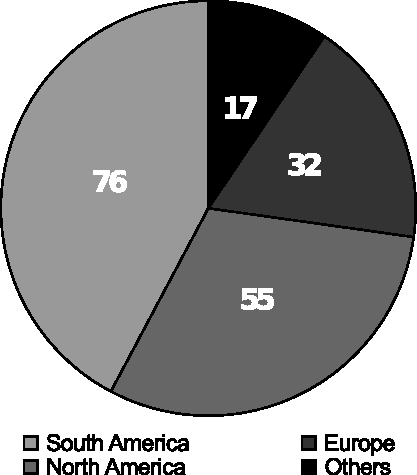
\includegraphics[scale=0.8]{floss-world.pdf}
    \caption{FLOSS answers in the world}
    \label{fig:floss-world}
  \end{minipage}
  \begin{minipage}[t]{0.5\linewidth}
    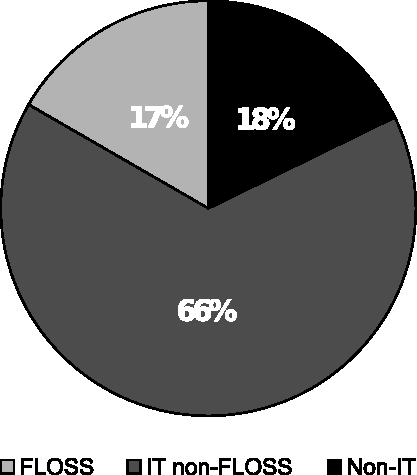
\includegraphics[scale=0.8]{floss-income.pdf}
    \caption{Main income origin for FLOSS participants}
    \label{fig:floss-income}
  \end{minipage}
\end{figure}

The analysis was performed over the 180 answers left since they
provided more interesting data. Figure \ref{fig:floss-world}
represents the distribution of the answers around the globe. Figure
\ref{fig:floss-income} shows the main income origin of the
participants. It is interesting to notice that those data do not
divert that much from the results collected from the FLOSS world
project mentioned previously.

The average age of the participants was 28 years old and the average
year of first FLOSS contribution was 2003. Figure
\ref{fig:floss-firstxp} shows that younger participants started
contributing earlier in their life than older participants which can
be explained by the increasing ease to get in touch with a computer in
the last years.

\begin{figure}[htb]
  \centering
  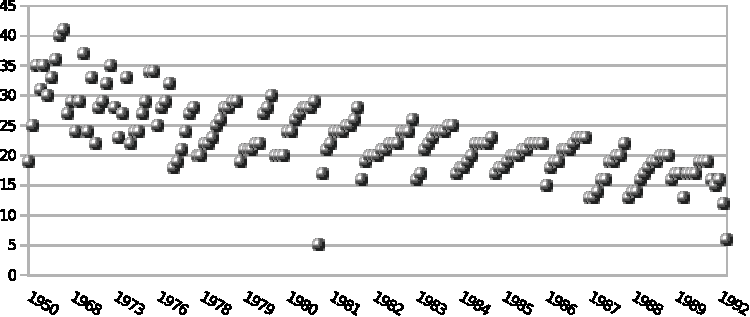
\includegraphics[scale=.9]{floss-firstxp.pdf}
  \caption{Age of first FLOSS contribution by year of birth}
  \label{fig:floss-firstxp}
\end{figure}
% TODO Melhorar gráfico de idades de contribuição inicial

About two thirds of the participants were project maintainers,
commiters or programmers. The last third was partitioned between other
roles as shows Figure \ref{fig:floss-roles}. Team sizes were also
fairly representative since only 6\% of the project were single person
team while 48\% were up to 5 team members. Figure
\ref{fig:floss-teams} shows those results and the reported team
sizes. It is interesting to notice that such profile is similar to the
one described by Reis \cite{reis2003} obtained in 2003.

\begin{figure}[htb]
  \begin{minipage}[t]{0.5\linewidth}
    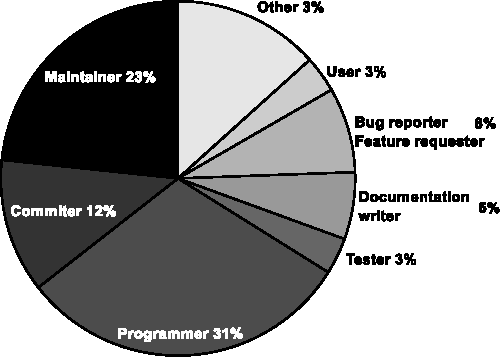
\includegraphics[scale=0.8]{floss-roles.pdf}
    \caption{Distribution of participant's roles}
    \label{fig:floss-roles}
  \end{minipage}
  \begin{minipage}[t]{0.5\linewidth}
    \begin{flushright}
      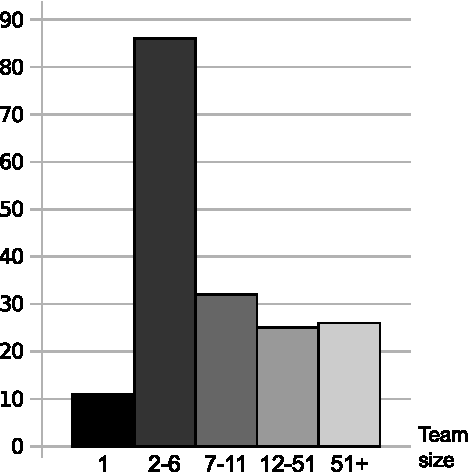
\includegraphics[scale=0.65]{floss-teams.pdf}
      \caption{FLOSS projects reported team sizes}
      \label{fig:floss-teams}
    \end{flushright}
  \end{minipage}
\end{figure}

Regarding the main communication channels, it seems to have changed a
little since the FLOSS world research or Reis' one. The main
communication channels with the rest of the team are still mailing
lists (27\%) and Internet Relay Chat (IRC - 23\%). However the amount
of people using face to face communication within the team shows some
increase (now at 15\%).

The evaluated quality of communication in those channels was fairly
similar. Mailing lists were evaluated to be 44\% effective against
52\% for IRC channels and 49\% for face to face. It seems with the
growing adoption of fast feedback channels over the Internet, mailing
lists are showing signs of weakness comparing to higher bandwidth
channels.

When it comes to communication with the users, mailing lists were the
most used (32\%) followed by websites (18\%) and IRC channels, emails
and issue trackers (11\% each). When it comes to quality of
communication in such channels, IRC channels scores once again with
49\% effectiveness against 44\% for mailing lists, 37\% for websites,
33\% for issue tracker and mere 23\% for emails.

For both environments, other communication channels were omitted since
there were too few answers to show any significant data.

\begin{figure}[htb]
  \centering
  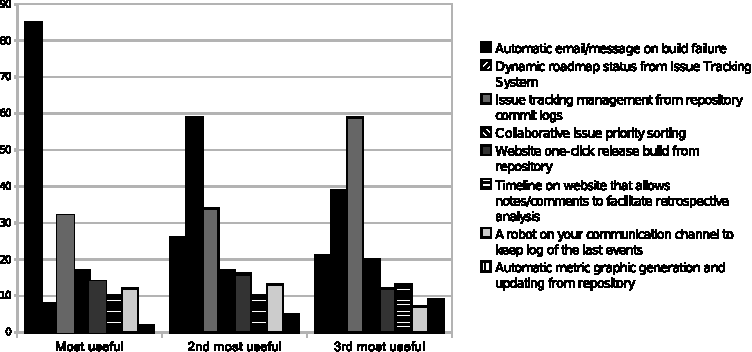
\includegraphics{floss-tools.pdf}
  \caption{FLOSS answers regarding tools usefulness}
  \label{fig:floss-tools}
\end{figure}

Figure \ref{fig:floss-tools} shows the top three choices of most
useful tools within a FLOSS project. Automatic email/message on build
failure was considered the most useful tool by large followed by a
dynamic roadmap status from the issue tracking system and issue
tracking management from repository commit logs.

\begin{figure}[hbt]
  \centering
  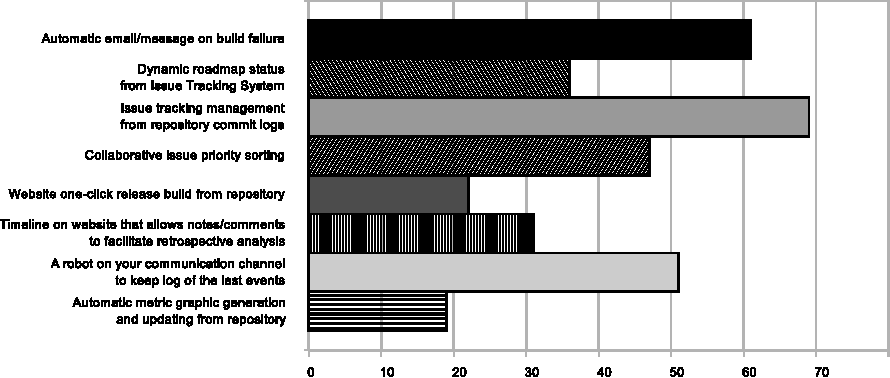
\includegraphics[scale=.8]{floss-existingtools.pdf}
  \caption{Tool participants already use in their FLOSS project}
  \label{fig:floss-existingtools}
\end{figure}

Figure \ref{fig:floss-existingtools} shows that a reasonable amount of
project already have automatic email/message on build failure and
issue track management from repository commit logs.  However, we
should be aware that Github features an issue tracking management from
repository commits while many other forges don't. And since Github
officially announced the survey, it is probable that many of their
users answered the survey. Therefore the sample could be biased in
such sense.

\subsection{Individual results from the Agile community}
\label{subsec:agile-results}

The results for the survey directed to the agile community were
collected between 2009/10/01 and 2009/12/01. It received 204 answers
from which 9 were duplicate entries and 34 were invalid due to the use
of incompatible browsers. Such data shows us that about 18\% of the
agile community still use browsers incompatible with Javascript
standards. Sensibly more people than in the FLOSS community.

Out of those 161 valid answers, only 28 were from people that never
actually participated in an agile project but considered themselves as
agile practitioners. Another fairly different result from the FLOSS
community. The agile community seems to value ``hands on'' experience
much more than the FLOSS community.

\begin{figure}[htb]
  \begin{minipage}[t]{0.5\linewidth}
    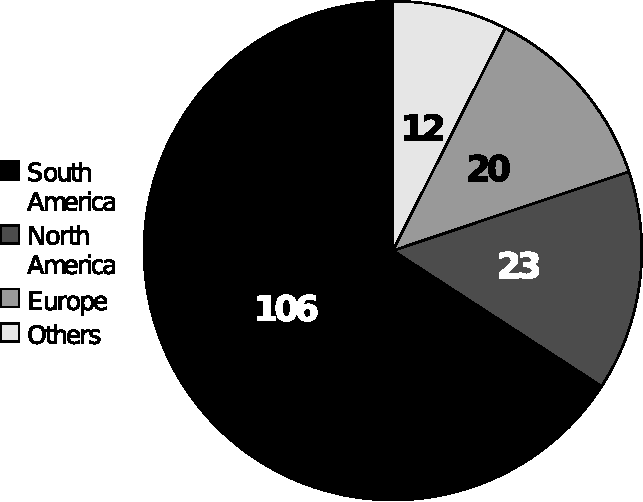
\includegraphics[scale=0.5]{agile-world.pdf}
    \caption{Answers to the agile survey by region of the world}
    \label{fig:agile-world}
  \end{minipage}
  \begin{minipage}[t]{0.5\linewidth}
    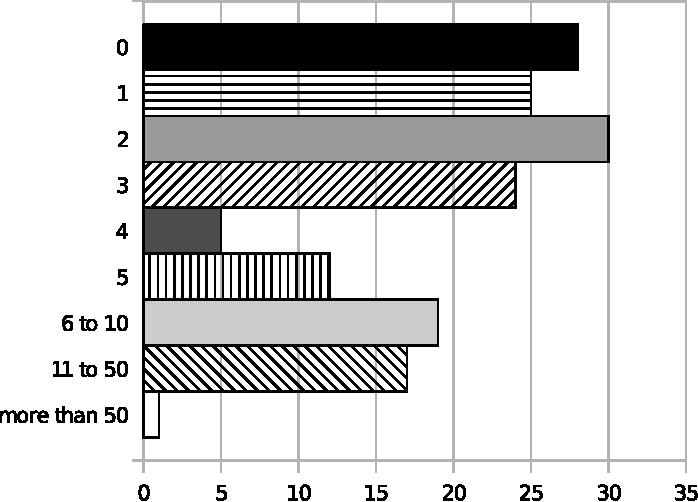
\includegraphics[scale=0.5]{agile-xp.pdf}
    \caption{Number of agile projects experience of the participants}
    \label{fig:agile-xp}
  \end{minipage}
\end{figure}

However it is not a very deep experience since 51\% of the
participants were involved in at most 2 agile projects and only 23\%
had more than 5 agile projects experience.  For the rest of the
analysis, participants without any agile experience will not be
counted since they provide little useful data.

Most participants with some experience only had a very recent contact
with agile projects. Figure \ref{fig:agile-distributed} shows that the
first experience with agile for most participants only happened after
2006. We can also see that there is a fairly regular amount of people
with distributed agile experience regardless of the year of first
agile experience which suggests there has not been a major increase on
distributed agile projects.

\begin{figure}[htb]
  \begin{minipage}[t]{0.55\linewidth}
    \centering
    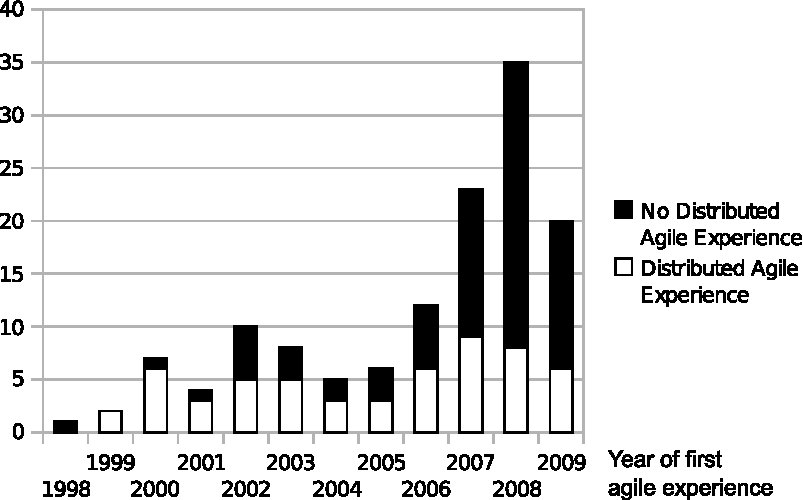
\includegraphics[scale=.45]{agile-distributed.pdf}
    \caption{Distributed agile experience according to the year of the
      first agile experience}
    \label{fig:agile-distributed}
  \end{minipage}
  \begin{minipage}[t]{0.45\linewidth}
    \centering
    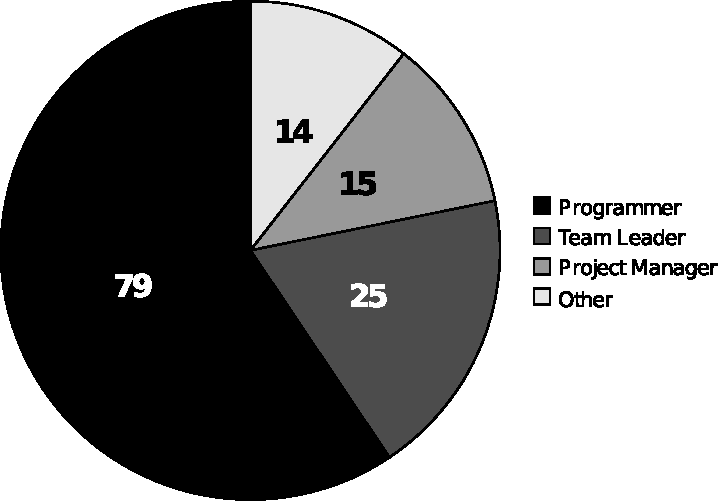
\includegraphics[scale=.45]{agile-roles.pdf}
    \caption{Roles description in the agile community}
    \label{fig:agile-roles}
  \end{minipage}
\end{figure}

Figure \ref{fig:agile-roles} shows that most participants considered
themselves programmers which contrasts with the variety of roles
accumulated in the FLOSS survey. Such indication can be justified by
the low hierarchy suggested by some agile books.
% TODO Ref

When it comes to team sizes, smaller teams are obviously
preferred. 37\% of the participants reported to work with an average
team size between 1 and 5 people. 46\% reported to have teams from 6
to 10 people, 13\% worked with 11 to 20 people and only 4\% reported
to work on teams with more than 20 people. Such data shows that agile
teams are clearly smaller teams still following the original
suggestions.

About 70\% of those teams have face to face communication with their
clients and evaluate the quality of such communication around
67\%. Emails, issue tracking systems and telephones accumulate another
19\% of the teams' communication with their clients with only 54\%,
50\% and 35\% effectiveness respectively. The rest of the channels are
not used enough to provide trustful data.

In distributed environments, the results show that there is no clear
consensus regarding the best communication channel within the
team. There is no clearly most used communication channel nor a
clearly most effective one. However, there is a clearly less effective
one. Emails share a reasonable part of the experiences but are rated
around 31\% effective to communicate between distributed teams which
ranks way below most reported channels.

The ineffectiveness of those communication channel can explain why
56\% of the participants stated that ``discovering what the
users/clients need/want'' is the biggest problem they face on their
agile projects. The second greatest problem is to ``synchronize with
other collaborators to achieve a common goal'' and to ``discover what
is the next task to be done''.

\begin{figure}[hbt]
  \centering
  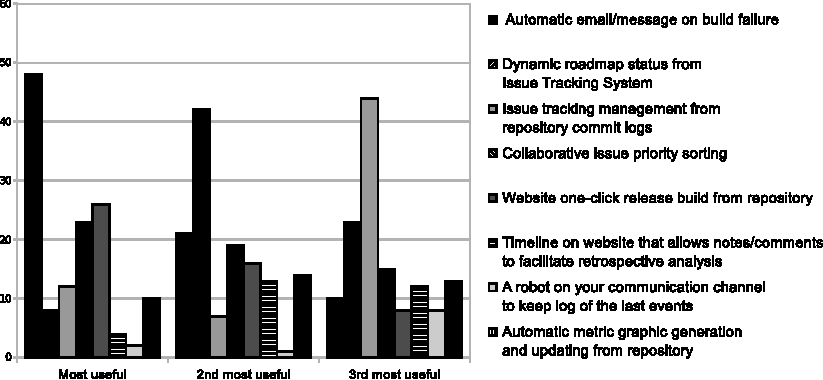
\includegraphics[scale=.8]{agile-tools.pdf}
  \caption{Most useful tools to agile practitioners}
  \label{fig:agile-tools}
\end{figure}

Regarding the useful tools to help agile practitioners, the results
are very similar to the ones listed by FLOSS contributors. The most
useful tools for agile practitioners are exactly the same as for FLOSS
contributors. Messages warning of build failures lead the ranking
followed by dynamic roadmaps and issue tracking management from commit
logs.

It is no surprise that for the 35\% of agilists that contribute to
FLOSS projects, the problems encountered in their FLOSS environments
are the same as in their agile environment. The tools to mitigate
their FLOSS problems are also the exact same ones from the agile
enviroment. However, such similarity does not come from the fact that
the projects in which agilists contribute are agile. Averagely, the
participants graded their FLOSS project to be only 56\% agile. Such
non agility with the similar results might indicate that agility and
FLOSS development have the same unsolved problems.

\section{Conclusion}
\label{sec:conclusion}

The results of the survey indicate that the communities are not very
closely related but share common problems and views to solve those
problems. It seems, however, that the most severe issues are not
directly addressed with the suggested tools.

%\subsubsection*{Ackowledgments.}

%This work was supported by the QualiPSo project \cite{url:qualipso}.

\begin{thebibliography}{5}

\bibitem{report:dempsey1999} Bert J Dempsey and Debra Weiss and Paul
  Jones and Jane Greenberg: A quantitative profile of a community of
  open source Linux developers (1999)

\bibitem{url:agilemanifesto} Kent Beck and Alistair Cockburn and Ward
  Cunningham and Martin Fowler and Ken Schwaber and al.: Manifesto for
  Agile Software Development, http://agilemanifesto.org (2001)

\bibitem{conference:oopsla2007} Dennis Mancl and Steven Fraser and
  William Opdyke: No silver bullet: a retrospective on the essence and
  accidents of software engineering (2007)

\bibitem{brooks1987} Frederick P. Brooks, Jr.: No Silver Bullet:
  Essence and Accidents of Software (1987)

\bibitem{gabriel2005} Ron Goldman and Richard P. Gabriel: Innovation
  Happens Elsewhere: Open Source as Business Strategy (2005)

\bibitem{XP2002} Kent Beck and Cynthia Andres: Extreme Programming
  Explained: Embrace Change, 2nd Edition (2004)

\bibitem{schwaber2004} Ken Schwaber: Agile Project Management with
  Scrum (2004)

\bibitem{cockburn2002} Alistair Cockburn: Agile Software Development
  (2002)

\bibitem{ohno1998} Taiichi Ohno: Toyota Production System: Beyond
  Large-Scale Production (1998)

\bibitem{poppendieck2005} Mary Poppendieck and Tom Poppendieck:
  Introduction to Lean Software Development (2005)

\bibitem{url:fowler2000orig} Martin Fowler: The New Methodology,
  http://martinfowler.com/articles/newMethodologyOriginal.html

\bibitem{fogel2005} Karl Fogel: Producing Open Source Software (2005)

\bibitem{url:flossproject} International Institute of Infonomics -
  University of Maastricht: Free/Libre/Open Source Software: Survey
  and Study - Report, http://www.flossproject.org/report/

\bibitem{url:flossdata} International Institute of Infonomics -
  University of Maastricht: Free/Libre/Open Source Software: Survey
  and Study - Report, http://www.flossproject.org/floss1/stats.html

\bibitem{reis2003} Christian Robottom Reis: Caracteriza\c{c}\~{a}o de
  um Processo de Software para Projetos de Software Livre (2003)

\bibitem{raymond1999} Eric S. Raymond: The Cathedral \& the Bazaar:
  Musings on {Linux} and Open Source by an Accidental Revolutionary
  (1999)

\bibitem{crowston2002} Kevin Crowston and Barbara Scozzi: Open source
  software projects as virtual organisations: competency rallying for
  software development (2002)

\bibitem{fitzgerald2000} Joseph Feller and Brian Fitzgerald: A
  framework analysis of the open source software development paradigm
  (2000)

\bibitem{warsta2002} Pekka Abrahamsson and Outi Salo and Jussi
  Ronkainen and Juhani Warsta: Agile software development methods
  (2002)

\bibitem{cockburn2004} Alistair Cockburn: Crystal Clear: A
  Human-Powered Methodology for Small Teams (2004)

  % \bibitem{oram2007} Andy Oram: Why Do People Write Free
  %   Documentation?  Results of a Survey (2007)

  % \bibitem{riehle2007} Dirk Riehle: The Economic Motivation of Open
  %   Source Software: Stakeholder Perspectives (2007)

  % \bibitem{sutherland2007} Jeff Sutherland and Anton Viktorov and
  %   Jack Blount and Nikolai Puntikov: Distributed Scrum: Agile
  %   Project Management with Outsourced Development Teams (2007)

  % \bibitem{maurer2002} Frank Maurer: Supporting Distributed Extreme
  %   Programming (2002)

  % \bibitem{url:beck2008} Kent Beck: Tools for Agility,
  %   http://www.microsoft.com/downloads/details.aspx?FamilyID=ae7e07e8-0872-47c4-b1e7-2c1de7facf96
  %   (2008)

  % \bibitem{nagappan2003} Nachiappan Nagappan and Prashant Baheti and
  %   Laurie Williams and Edward Gehringer and David Stotts: Virtual
  %   Collaboration through Distributed Pair Programming (2003)

  % \bibitem{url:north2006} Dan North: Behaviour Driven Development,
  %   http://dannorth.net/introducing-bdd

  % \bibitem{sato2007} Danilo Sato and Alfredo Goldman and Fabio Kon:
  %   Tracking the Evolution of Object-Oriented Quality Metrics on
  %   Agile Projects (2007)

  % \bibitem{surowiecki2004} J. Surowiecki: The Wisdom of Crowds: Why
  %   the many are smarter than the few and how collective wisdom
  %   shapes business, economies, societies, and nations (2004)

  % \bibitem{tapscott2006} Don Tapscott and Anthony D. Williams:
  %   Wikinomics: How Mass Collaboration Changes Everything (2006)

  % \bibitem{benkler2006} Yochai Benkler: The Wealth of Networks: How
  %   Social Production Transforms Markets and Freedom (2006)

%\bibitem{url:qualipso} Qualipso | Trust and Quality in Open Source
%  systems, http://www.qualipso.org/
\end{thebibliography}

\appendix
\section{Paper version of the survey to the FLOSS community}
\label{appendix:a}

\begin{enumerate}
\item What country do you live in? \verb=_________________=
  \vspace{8pt}

\item What year where you born? \verb=______= \vspace{8pt}

\item How many FLOSS projects have you already contributed with?

  \verb=( ) 0 ( ) 1 ( ) 2 ( ) 3 ( ) 4 ( ) 5-10 ( ) 11-50 ( ) 51+=
  \vspace{8pt}

\item What is the FLOSS project you mostly contribute/contributed with? \verb= ______________= \vspace{0pt}

\item In which year was your first contribution to that project?
  \verb=______= \vspace{8pt}

\item What is/was your main role in that project?
  \begin{itemize}
    \begin{minipage}[t]{0.5\linewidth}
    \item[( ) ] Maintainer
    \item[( ) ] Commiter
    \item[( ) ] Programmer
    \item[( ) ] Tester
    \end{minipage}
    \begin{minipage}[t]{0.5\linewidth}
    \item[( ) ] Documentation writer
    \item[( ) ] Bug reporter/Feature requester
    \item[( ) ] User
    \item[( ) ] Other: \verb=_________________=
    \end{minipage}
  \end{itemize}
  \vspace{8pt}

\item Do/Did you receive any income from your FLOSS contributions?
  \verb=( ) Yes ( ) No= \vspace{0pt}

\item If you do/did, is/was this your main income?
  \verb=( ) Yes ( ) No= \vspace{8pt}

\item If you answered no to the previous question or the one before,
  is/was your main income related to IT?  \verb=( ) Yes ( ) No=
  \vspace{8pt}

\item How many people work (or worked) with you on your main FLOSS
  project?  \verb=( ) 0 ( ) 1-5 ( ) 6-10 ( ) 11-50 ( ) 51+=
  \vspace{8pt}

\item What is/was the main communication channel with the team of that
  project?
  \begin{itemize}
    \begin{minipage}[t]{0.5\linewidth}
    \item[( ) ] Face to face
    \item[( ) ] Website
    \item[( ) ] Mailing list
    \item[( ) ] Issue tracker (Trac, Bugzilla, etc.)
    \item[( ) ] Internet Relay Chat (IRC)
    \end{minipage}
    \begin{minipage}[t]{0.5\linewidth}
    \item[( ) ] Instant Message (Jabber, ICQ, etc.)
    \item[( ) ] Email
    \item[( ) ] VoIP (Skype, Ekiga, iChat, etc.)
    \item[( ) ] None
    \item[( ) ] Other: \verb=_____________=
    \end{minipage}
  \end{itemize}
  \vspace{8pt}

\item How would you evaluate the quality of your communication with
  that team?

  Extremely poor \verb=---------------------------------------=
  Perfect \vspace{8pt}

\item What is/was the main communication channel with the users of
  that project?
  \begin{itemize}
    \begin{minipage}[t]{0.5\linewidth}
    \item[( ) ] Face to face
    \item[( ) ] Website
    \item[( ) ] Mailing list
    \item[( ) ] Issue tracker (Trac, Bugzilla, etc.)
    \item[( ) ] Internet Relay Chat (IRC)
    \end{minipage}
    \begin{minipage}[t]{0.5\linewidth}
    \item[( ) ] Instant Message (Jabber, ICQ, etc.)
    \item[( ) ] Email
    \item[( ) ] VoIP (Skype, Ekiga, iChat, etc.)
    \item[( ) ] None
    \item[( ) ] Other: \verb=_____________=
    \end{minipage}
  \end{itemize}
  \vspace{8pt}

\item How would you evaluate the quality of your communication with
  the users?

  Extremely poor \verb=---------------------------------------=
  Perfect \vspace{8pt}

\item How much effort do/did you spend to keep project's information
  updated?

  Very little \verb=---------------------------------------= Huge
  \vspace{8pt}

\item Which of the following tools does/did your project already use?
  \begin{itemize}
  \item[[ ] ] Automatic email/message on build failure
  \item[[ ] ] Dynamic roadmap status from Issue Tracking System
  \item[[ ] ] Issue tracking management from repository commit logs
  \item[[ ] ] Website one-click release build from repository
  \item[[ ] ] Automatic metric graphic generation and updating from
    repository
  \item[[ ] ] Collaborative issue priority sorting
  \item[[ ] ] Timeline on website that allows notes/comments to
    facilitate retrospective analysis
  \item[[ ] ] A robot on your communication channel to keep log of the
    last events
  \end{itemize}
  \vspace{8pt}

\item Sort the tools from the most useful (first) to the less useful
  (last).
  \begin{itemize}
  \item[( ) ] Automatic email/message on build failure
  \item[( ) ] Dynamic roadmap status from Issue Tracking System
  \item[( ) ] Issue tracking management from repository commit logs
  \item[( ) ] Website one-click release build from repository
  \item[( ) ] Automatic metric graphic generation and updating from
    repository
  \item[( ) ] Collaborative issue priority sorting
  \item[( ) ] Timeline on website that allows notes/comments to
    facilitate retrospective analysis
  \item[( ) ] A robot on your communication channel to keep log of the
    last events
  \end{itemize}
\end{enumerate}

\section{Paper version of the survey to the agile community}
\label{appendix:b}

\begin{enumerate}
\item What country do you live in? \verb=_________________=
  \vspace{8pt}

\item What year where you born? \verb=______= \vspace{8pt}

\item How many projects you would consider agile have you been on?

  \verb=( ) 0 ( ) 1 ( ) 2 ( ) 3 ( ) 4 ( ) 5-10 ( ) 11-50 ( ) 51+=
  \vspace{8pt}

\item In which year was the first Agile project you participated?
  \verb=______= \vspace{8pt}

\item What is/was your main role in that project?
  \begin{itemize}
    \begin{minipage}[t]{0.5\linewidth}
    \item[( ) ] Project manager
    \item[( ) ] Team leader
    \item[( ) ] Programmer
    \item[( ) ] Quality Analyst
    \end{minipage}
    \begin{minipage}[t]{0.5\linewidth}
    \item[( ) ] Tester
    \item[( ) ] Tracker
    \item[( ) ] Documenter
    \item[( ) ] Other: \verb=_________________=
    \end{minipage}
  \end{itemize}
  \vspace{8pt}

\item What is/was the average number of people in the agile
  projects you worked?
  \verb=( ) 1-5 ( ) 6-10 ( ) 11-20 ( ) 21-50 ( ) 51-100 ( )100+=
  \vspace{8pt}

\item What is/was your main communication channel with the
  clients of that project?
  \begin{itemize}
    \begin{minipage}[t]{0.5\linewidth}
    \item[( ) ] Face to face
    \item[( ) ] Website
    \item[( ) ] Mailing list
    \item[( ) ] Issue tracker (Trac, Bugzilla, etc.)
    \item[( ) ] Internet Relay Chat (IRC)
    \item[( ) ] Other: \verb=_____________=
    \end{minipage}
    \begin{minipage}[t]{0.5\linewidth}
    \item[( ) ] Instant Message (Jabber, ICQ, etc.)
    \item[( ) ] Email
    \item[( ) ] Telephone
    \item[( ) ] VoIP (Skype, Ekiga, iChat, etc.)
    \item[( ) ] None
    \end{minipage}
  \end{itemize}
  \vspace{8pt}

\item How would you evaluate the quality of your communication with
  the clients?

  Extremely poor \verb=---------------------------------------=
  Perfect \vspace{8pt}

\item Have you ever been on a distributed agile project?
  \verb=( ) Yes ( ) No= \vspace{8pt}

\item What is/was the main communication channel within
  that distributed team?
  \begin{itemize}
    \begin{minipage}[t]{0.5\linewidth}
    \item[( ) ] Face to face
    \item[( ) ] Website
    \item[( ) ] Mailing list
    \item[( ) ] Issue tracker (Trac, Bugzilla, etc.)
    \item[( ) ] Internet Relay Chat (IRC)
    \item[( ) ] Other: \verb=_____________=
    \end{minipage}
    \begin{minipage}[t]{0.5\linewidth}
    \item[( ) ] Instant Message (Jabber, ICQ, etc.)
    \item[( ) ] Email
    \item[( ) ] Telephone
    \item[( ) ] VoIP (Skype, Ekiga, iChat, etc.)
    \item[( ) ] None
    \end{minipage}
  \end{itemize}
  \vspace{8pt}

\item If you had distributed agile experience, how would you evaluate
  the quality of your communication with that team?

  Extremely poor \verb=---------------------------------------=
  Perfect \vspace{8pt}

\item For some of the common problems encountered by agile teams
  listed below, sort the 3 most critical problems in the agile
  environments you worked on.
  \begin{itemize}
  \item[[ ] ] Discover what the users/clients need/want
  \item[[ ] ] Discover what is the next task to be done
  \item[[ ] ] Understand how the project works from a technical point
    of view
  \item[[ ] ] Discover the current project status
  \item[[ ] ] Integrate the source code to the main repository
  \item[[ ] ] Keep the information about the project updated in its
    main communication channel
  \item[[ ] ] Evaluate the work done to identify improvement points
  \item[[ ] ] Synchronize with other collaborators to achieve a common
    goal
  \end{itemize}
  \vspace{8pt}

\item Sort the 3 tools that would most help you in a distributed agile
  environment.
  \begin{itemize}
  \item[[ ] ] Automatic email/message on build failure
  \item[[ ] ] Dynamic roadmap status from Issue Tracking System
  \item[[ ] ] Issue tracking management from repository commit logs
  \item[[ ] ] Website one-click release build from repository
  \item[[ ] ] Automatic metric graphic generation and updating from
    repository
  \item[[ ] ] Collaborative issue priority sorting
  \item[[ ] ] Timeline on website that allows notes/comments to
    facilitate retrospective analysis
  \item[[ ] ] A robot on your communication channel to keep log of the
    last events
  \end{itemize}
\vspace{8pt}

\item Have you ever contributed to Free, Libre, Open Source Software
  (FLOSS)?  \verb=( ) Yes ( ) No= \vspace{8pt}

\item How would you evaluate the agile level of your FLOSS project?

  Anti agile \verb=---------------------------------------= Very agile
  \vspace{8pt}

\item For some of the common problems encountered by agile teams
  listed below, sort the 3 most critical problems in the FLOSS
  projects you worked on.
  \begin{itemize}
  \item[[ ] ] Discover what the users/clients need/want
  \item[[ ] ] Discover what is the next task to be done
  \item[[ ] ] Understand how the project works from a technical point
    of view
  \item[[ ] ] Discover the current project status
  \item[[ ] ] Integrate the source code to the main repository
  \item[[ ] ] Keep the information about the project updated in its
    main communication channel
  \item[[ ] ] Evaluate the work done to identify improvement points
  \item[[ ] ] Synchronize with other collaborators to achieve a common
    goal
  \end{itemize}
  \vspace{8pt}

\item Sort the 3 tools that would most help you in that FLOSS
  environment.
  \begin{itemize}
  \item[[ ] ] Automatic email/message on build failure
  \item[[ ] ] Dynamic roadmap status from Issue Tracking System
  \item[[ ] ] Issue tracking management from repository commit logs
  \item[[ ] ] Website one-click release build from repository
  \item[[ ] ] Automatic metric graphic generation and updating from
    repository
  \item[[ ] ] Collaborative issue priority sorting
  \item[[ ] ] Timeline on website that allows notes/comments to
    facilitate retrospective analysis
  \item[[ ] ] A robot on your communication channel to keep log of the
    last events
  \end{itemize}
\end{enumerate}
\end{document}
